\subsection{Canal BSC em cascata com apagamento}
\begin{questions}
% resource/HW4_ES250_sol_a.pdf
\question{
Suponha que um canal binário simétrico de capacidade $C_1$ seja imediatamente 
seguido de um canal binário com apagamento e capacidade $C_2$.
Determine a capacidade $C$ do canal resultante.

}

\begin{solution}

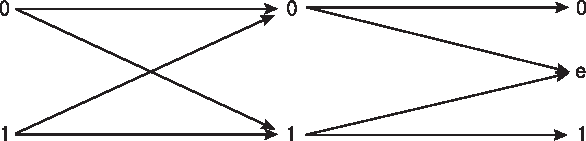
\includegraphics[width=0.5\textwidth]{../images/canalbinapag.pdf}

Seja $C_1 = 1 - H(p)$ a capacidade do canal binário simétrico, com parâmetro $p$, e
$C_2 = 1 - \alpha$ a capacidade do canal binário com apagamento, com parâmetro $\alpha$.
Seja $\tilde{Y}$ a saída do canal final (cascata dos dois canais), e seja $Y$ a saída 
do canal binário simétrico. A regra de transição para o canal final em cascata é dado por
\begin{equation}
p(\tilde{y}|x) = \sum_{y=0,1} p(\tilde{y}|y) p(y|x)
\end{equation}
para cada par $(x,\tilde{y})$.

Temos então a seguinte matriz de transição
\begin{equation}
  p(\tilde{y} \vert x) = 
\begin{blockarray}{cccc}
 0 & e & 1  \\
\begin{block}{(ccc)c}
  (1-p)(1-\alpha) & \alpha & p(1-\alpha)     & 0 \\
  p(1-\alpha)     & \alpha & (1-p)(1-\alpha) & 1 \\
\end{block}
\end{blockarray}
\label{eqmatq8}
\end{equation}
Note que as linhas desta matriz são permutação uma das outra, mas
a soma de cada coluna é diferente. Por tanto, esta matriz não é fracamente simétrica\footnote{
  Um canal é simétrico se as linhas da matriz de transmissão $p(y|x)$ são permutação uma das outras,
  e as colunas desta matriz também são permutação uma das outras. Um canal é fracamente simétrico
  se cada linha da matriz for uma permutação das outras linhas e todas as colunas tiverem a mesma
  soma $\sum_x p(y|x)$. Para canais fracamente simétricos teremos 
  $C = \log \vert \mathcal{Y} \vert - H(r)$, onde $r$ é a linha da matriz de transmissão.
}. 

Seja $X \sim \text{Bern}(\pi)$ a entrada do canal, então
\begin{eqnarray}
C &=& \max_{p(x)} I(X;\tilde{Y}) \nonumber \\
        &=& \max_{\pi} \left( H(\tilde{Y}) - H(\tilde{Y}|X) \right) \nonumber \\
        &=& \max_{\pi} \left( H(\tilde{Y}) \right) - H(\tilde{Y}|X) 
\end{eqnarray}
Dada a matriz de transição, podemos calcular $H(\tilde{Y}|X)$.
\begin{eqnarray}
H(\tilde{Y}|X) &=& H\left( (1-p)(1-\alpha), \alpha, p(1-\alpha) \right) \nonumber \\
        &=& (1-p)(1-\alpha) \log \left( (1-p)(1-\alpha) \right) - \alpha \log \alpha - p(1-\alpha) \log \left( p(1-\alpha) \right) \nonumber \\
        &=& (1-\alpha) \left( (1-p) \log (1-p) - p \log p \right) - (1-\alpha) \log (1-\alpha) \underbrace{\left( (1-p) + p \right)}_{=1} - \alpha \log \alpha \nonumber \\
        &=& (1-\alpha) H(p) + H(\alpha)
\end{eqnarray}


Ainda precisamos analisar $H(\tilde{Y})$ para calcular $C$. Precisamos então determinar $p(\tilde{y})$.
\begin{eqnarray}
p(\tilde{y} = 0) &=& p(\tilde{y} = 0, x = 0) + p(\tilde{y} = 0, x = 1) \nonumber \\
        &=& p(\tilde{y} = 0 | x = 0) p(x = 0) + p(\tilde{y} = 0 | x = 1) p(x = 1) \nonumber \\
        &=& (1-p)(1-\alpha) \pi + p(1-\alpha)(1-\pi) \nonumber \\
        &=& (1-\alpha) \left( (1-p)\pi + p(1-\pi) \right) \\
p(\tilde{y} = e) &=& p(\tilde{y} = e, x = 0) + p(\tilde{y} = e, x = 1) \nonumber \\
        &=& p(\tilde{y} = e | x = 0) p(x = 0) + p(\tilde{y} = e | x = 1) p(x = 1) \nonumber \\
        &=& \alpha \pi + \alpha (1 - \pi) = \alpha \\
p(\tilde{y} = 1) &=& p(\tilde{y} = 1, x = 0) + p(\tilde{y} = 1, x = 1) \nonumber \\
        &=& p(\tilde{y} = 1 | x = 0) p(x = 0) + p(\tilde{y} = 1 | x = 1) p(x = 1) \nonumber \\
        &=& p(1-\alpha) \pi + (1-p)(1-\alpha)(1-\pi) \nonumber \\
        &=& (1-\alpha) \left( p\pi + (1-p)(1-\pi) \right)
\end{eqnarray}
e assim teremos que 
\begin{equation}
H(\tilde{Y}) = H\left( (1-\alpha)(\pi(1-p)+p(1-\pi)), \alpha , (1-\alpha)(p\pi + (1-p)(1-\pi) ) \right) .
\end{equation}
Para maximizar $H(\tilde{Y})$, basta fazer $p(\tilde{y} = 0) = p(\tilde{y} = 1)$, uma vez que 
$p(\tilde{y} = e)$ depende apenas de $\alpha$.
\begin{eqnarray}
(1-\alpha) \left( (1-p)\pi + p(1-\pi) \right) &=& (1-\alpha) \left( p\pi + (1-p)(1-\pi) \right) \nonumber \\
\pi -p\pi + p - p\pi &=& p\pi + 1 - \pi - p + p\pi \nonumber \\
2\pi (1 - 2p) &=& 1 - 2p \nonumber \\
\pi &=& \frac{1}{2}
\end{eqnarray}
Podemos então calcular o valor máximo de $H(\tilde{Y})$.
\begin{eqnarray}
H(\tilde{Y}) &=& H\left( (1 - \alpha)(\frac{1}{2} - \frac{1}{2}p + \frac{1}{2}p) , \alpha , (1 - \alpha)(\frac{1}{2}p + \frac{1}{2} - \frac{1}{2}p ) \right) \nonumber \\
        &=& H\left( (1 - \alpha) \frac{1}{2} , \alpha , (1 - \alpha) \frac{1}{2} \right) \nonumber \\
        &=& - 2 \frac{1}{2} (1 - \alpha) \log \left( \frac{1}{2} (1 - \alpha) \right) - \alpha \log \alpha \nonumber \\
        &=& -(1-\alpha) \log (1-\alpha) + (1-\alpha) \log 2 - \alpha \log \alpha \nonumber \\
        &=&  (1-\alpha) + H(\alpha)
\end{eqnarray}
A capacidade do canal então será
\begin{eqnarray}
C &=& \max_{\pi} \left( H(\tilde{Y}) \right) - H(\tilde{Y}|X) \nonumber \\
        &=& (1-\alpha) + H(\alpha) - ( (1-\alpha) H(p) + H(\alpha) ) \nonumber \\
        &=& \underbrace{(1-\alpha)}_{C_2} \underbrace{(1 - H(p))}_{C_1} \nonumber \\
        &=& C_1 C_2
\end{eqnarray}



\end{solution}
\end{questions}

